% Template for Cogsci submission with R Markdown

% Stuff changed from original Markdown PLOS Template
\documentclass[10pt, letterpaper]{article}

\usepackage{cogsci}
\usepackage{pslatex}
\usepackage{float}
\usepackage{caption}

% amsmath package, useful for mathematical formulas
\usepackage{amsmath}

% amssymb package, useful for mathematical symbols
\usepackage{amssymb}

% hyperref package, useful for hyperlinks
\usepackage{hyperref}

% graphicx package, useful for including eps and pdf graphics
% include graphics with the command \includegraphics
\usepackage{graphicx}

% Sweave(-like)
\usepackage{fancyvrb}
\DefineVerbatimEnvironment{Sinput}{Verbatim}{fontshape=sl}
\DefineVerbatimEnvironment{Soutput}{Verbatim}{}
\DefineVerbatimEnvironment{Scode}{Verbatim}{fontshape=sl}
\newenvironment{Schunk}{}{}
\DefineVerbatimEnvironment{Code}{Verbatim}{}
\DefineVerbatimEnvironment{CodeInput}{Verbatim}{fontshape=sl}
\DefineVerbatimEnvironment{CodeOutput}{Verbatim}{}
\newenvironment{CodeChunk}{}{}

% cite package, to clean up citations in the main text. Do not remove.
\usepackage{apacite}

% KM added 1/4/18 to allow control of blind submission
\cogscifinalcopy

\usepackage{color}

% Use doublespacing - comment out for single spacing
%\usepackage{setspace}
%\doublespacing


% % Text layout
% \topmargin 0.0cm
% \oddsidemargin 0.5cm
% \evensidemargin 0.5cm
% \textwidth 16cm
% \textheight 21cm

\title{`Five' is the number of bunnies and hats: Children's
understanding of cardinal extension and exact number}

\setlength{\belowcaptionskip}{-10pt}

\author{{\large \bf Khuyen N. Le}, {\large \bf Christine Kwon}, {\large \bf Mincong Wu}, and {\large \bf David Barner} \\ \{knl005, ckwon, miw036, dbarner\}@ucsd.edu \\ Department of Psychology, University of California, San Diego \\ La Jolla, CA 92093, USA}

\newlength{\cslhangindent}
\setlength{\cslhangindent}{1.5em}
\newenvironment{CSLReferences}%
  {}%
  {\par}

\begin{document}

\maketitle

\begin{abstract}
When do children understand that number words (such as `five') refer to
exact quantities and that the same number word can be used to label two
sets whose items correspond 1-to-1 (e.g., if each bunny has a hat, and
there are five hats, then there are five bunnies)? Two studies with
English-speaking 2- to 5-year-olds revealed that children who could
accurately count large sets (CP knowers) were able to infer that sets
exhibiting 1-to-1 correspondence share the same number word, but not
children who could not accurately count large sets (subset knowers).
However, not all CP knowers made this inference, suggesting that
learning to construct and label large sets is a critical but
insufficient step in discovering that numbers represent exact
quantities. CP knowers also failed to identify 1-to-1 corresponding sets
when faced with sets that had an off-by-one difference, suggesting that
children who could accurately count large sets used approximate
magnitude to establish set equality, rather than 1-to-1 correspondence.
These results suggest that children's initial intuitions about numerical
and set equality are based on approximation, not 1-to-1 correspondence,
and that this occurs well after they have learned to count and construct
large sets.

\textbf{Keywords:}
number words; number concepts; exact equality; 1-to-1 correspondence;
cardinal extension; language development
\end{abstract}

\hypertarget{introduction}{%
\section{Introduction}\label{introduction}}

Imagine you attend a popular conference talk where every chair is
occupied. After the talk, you want to know how many people attended. Is
there a way to know? As numerate adults, we know that we can count the
number of chairs to infer the number of attendees. Understanding this
principle, sometimes called ``cardinal extension'', involves two
distinct abilities. First, it requires the non-linguistic ability to
recognize that two sets have the same number of items if and only if
their members can be placed in one-to-one correspondence, sometimes
called ``Hume's Principle'' (Boolos, 1986; Decock, 2008; Frege, 1880,
1884). Second, it requires understanding that a particular number word
can be applied to two different sets if and only if they have an equal
number of items. Therefore, cardinal extension integrates both
non-linguistic reasoning about exact equality and linguistic knowledge
of how number words encode number

How do children acquire this knowledge? According to one view, once
children learn their first 1-2 number words, they quickly infer that all
number words denote unique, exact, numerosities. Previous studies
establish that, beginning sometime after the age of 2, children learn
the meanings of the words `one', `two', and `three' one at a time over
the course of 1-2 years, during which time they are known as ``subset
knowers'' (since they know the meanings of only a subset of numbers,
e.g., Wynn, 1990, 1992). According to Sarnecka \& Gelman (2004),
knowledge of these first few number word meanings might be sufficient to
support an inference that all number words denote unique, exact,
numerosities, and therefore that sets which differ in number should
receive different numerical labels, while equinumerous sets should
receive the same labels. In support of this hypothesis, Sarnecka \&
Gelman (2004) presented subset knowers with a set labeled with a number
word (``Look, there are five frogs''), and found that when an item was
added or subtracted from the set, children judged that a different
number word should be used. Children also correctly reasoned that the
same number word should be used when the transformation did not change
the quantity, such as shaking the box containing the items. Notably,
these judgments extended to number words beyond subset knowers'
performance in a Give-N task, but not to other quantifiers such as `a
lot'. Other studies, however, have questioned these findings, showing
that children fail with highly similar tasks (Condry \& Spelke, 2008;
Sarnecka \& Wright, 2013), and that simpler explanations that do not
involve exact number knowledge can explain the data, including pragmatic
inferences like the principle of contrast (Brooks et al., 2013; see
Izard et al., 2014 for a discussion).

According to an alternative hypothesis, children only understand that
number words denote unique, exact, numerosities when they can construct
and provide the cardinal label for any sets they can count (Carey, 2004,
2009; Condry \& Spelke, 2008; Sarnecka \& Wright, 2013). Sometime after
they learn the meanings of `one', `two', and `three', children appear to
discover that counting can be used to both construct large sets and
label their cardinalities, at which point they are sometimes called
``Cardinal Principle'' knowers (or CP knowers). According to some
proposals, learning to accurately count and construct large sets
establishes children's understanding of how number words represent
cardinality. This is because mastery of counting requires establishing
1-to-1 correspondence between labels and counted objects, thus
guaranteeing that any counts to a particular number - like five - will
result in the same quantity (Carey, 2004, 2009). As evidence for this,
previous studies have found that CP knowers outperform subset knowers in
tests of cardinal extension. When shown two sets that appear equal in
number, CP knowers often correctly extend a number word (e.g., `five')
that labels one set to the other, while subset knowers fail at the same
task (Sarnecka \& Gelman, 2004; Sarnecka \& Wright, 2013). Similarly,
when shown a set of items labeled with a number word, e.g., `four
turtles', and asked to distinguish between two sets to find a set with
the same number word label, CP knowers, but not subset knowers, succeed
(Slusser \& Sarnecka, 2011).

However, some have suggested that the ability to accurately count and
label large sets may reflect rote procedures (Davidson et al., 2012),
and that many CP knowers still don't understand that every number word
denotes a unique cardinality, or that equinumerous sets should receive
the same cardinal label. As evidence for this, although CP knowers
outperform subset knowers on tests of cardinal extension, they rarely
perform at ceiling, failing from 15\% to 40\% of the trials depending of
the task (Sarnecka \& Gelman, 2004; Sarnecka \& Wright, 2013; Slusser \&
Sarnecka, 2011). In fact, multiple past studies report variability on
tests of cardinal extension until up to 5 years of age (Frydman \&
Bryant, 1988; Muldoon et al., 2003, 2005; Sophian et al., 1995). Adding
to doubt that children master cardinal extension when they become CP
knowers is the fact that children as old as 6 (beyond the age most
children in Western, English-speaking contexts become CP knowers) often
fail on tasks that test non-verbal understanding of 1-to-1
correspondence (Piaget, 1965; Russac, 1978; Schneider et al., 2022).

To summarize, previous studies have debated when and how children
acquire cardinal extension - i.e., understanding that two equal sets
should receive the same label, and that two sets are equal only if their
elements stand in 1-to-1 correspondence. Some argue that this knowledge
emerges after children learn just 1-2 small number words, while others
argue that it develops when children become CP knowers, or even sometime
after this. Critically, however, previous studies testing cardinal
extension are limited in various ways that make it difficult to know how
such knowledge actually arises. First, some studies found variability in
cardinal extension understanding between the ages of 3 and 5, but did
not assess children's understanding of counting or the CP, leaving open
the question of what role CP knowledge plays in cardinal extension
understanding (e.g., Frydman \& Bryant, 1988; Muldoon et al., 2003,
2005; Sophian et al., 1995). Second, other studies have classified
children as subset knowers or CP knowers and tested differences between
these groups, but have not analyzed sources of individual differences
between children within these groups (e.g., Sarnecka \& Gelman, 2004;
Sarnecka \& Wright, 2013; Slusser \& Sarnecka, 2011). Third, while
cardinal extension requires two components (recognizing equinumerous
sets and understanding that such sets share the same number label),
previous studies typically test only one or the other, but rarely test
both. Crucially, most studies that attempt to test both children's
reasoning about equinumerosity and how they use this knowledge to extend
number labels (e.g., Sarnecka \& Gelman, 2004) do not differentiate
between reasoning about exact vs.~approximate representations of number.
This is important, because children might represent two sets as ``the
same'' using approximate representations of number (ANS, Cordes et al.,
2001; Feigenson et al., 2004; Whalen et al., 1999), even if the sets
violate 1-to-1 correspondence and differ by 1 item. Consequently, to be
sure that children extend number words to sets that are exactly equal,
it's critical to ensure that their extension is not based on approximate
matches between sets.

The present studies aimed to address the limitations of past reports. We
presented subset knowers and CP knowers with two sets of animals in
unequal numbers (e.g., 5 bunnies and 7 lions). Animals in each group
carried items (e.g., the bunnies had blue hats and the lions had red
hats), such that the number of items was exactly equal to the number of
animals in each group. One set (e.g., the bunnies) was then hidden, and
children were prompted to infer how many animals were hidden. We asked
whether they would count the correct visible objects (e.g., the bunnies'
hats) to infer the number of hidden animals, compatible with knowledge
that two sets have the same number of items - and deserve the same
numerical label - if they stand in 1-to-1 correspondence. In Study 2, we
provided a stronger test of whether children who succeed in reasoning
about set equality do so through reasoning about exact equality or
approximate magnitudes. To do so, we contrasted a condition that
required reasoning about 1-to-1 correspondence vs.~a condition that
could be solved using approximate number knowledge. We report the main
results of these studies for the purposes of this short paper. Readers
are encouraged to refer to Le et al. (2024) for a more comprehensive
analysis and additional discussion.

\hypertarget{study-1-when-does-childrens-understanding-of-cardinal-extension-develop}{%
\section{Study 1: When does children's understanding of cardinal
extension
develop?}\label{study-1-when-does-childrens-understanding-of-cardinal-extension-develop}}

\hypertarget{methods}{%
\subsection{Methods}\label{methods}}

\hypertarget{participants}{%
\subsubsection{Participants}\label{participants}}

A preregistration is available at \url{https://osf.io/3v2cn}.
Eighty-four\footnote{We recruited four more CP knowers than
  preregistered due to an initial knower-level coding error.} children
were recruited from preschools in the US and Canada, and a children's
museum in the US. All participants spoke English as a primary language.
Based on preregistered criteria, we excluded two participants who did
not provide a response for more than one trial of the Cardinal Extension
task, and two trials due to experimenter error. Our final sample
included 82 children, with 38 subset knowers (23F, 15M; \(M_{age}\) =
3.55 {[}2.13; 5.20{]}; \(SD_{age}\) = 0.76) and 44 CP knowers (25F, 19M;
\(M_{age}\) = 4.63 {[}3.08; 5.95{]}; \(SD_{age}\) = 0.65).

\hypertarget{materials-procedure}{%
\subsubsection{Materials \& Procedure}\label{materials-procedure}}

All materials, data, and analysis code for Studies 1 and 2 are available
at \url{https://osf.io/eswa4}.

\vspace{10pt}

\noindent \textbf{\emph{Give-N.}} Participants were given a titrated
Give-N task (following the procedure in Wynn, 1992) to assess their
understanding of the CP. Participants were shown a box with fish and a
plate, and were asked to ``put N fish on the plate'' All participants
started with `five', received increasingly higher numbers (\(N\)+1, up
to `six') if they succeeded and lower numbers (\(N\)-1) if they failed.
We recorded the highest number for which a participant can construct
correct sets two out of three times. If the child constructed the wrong
set, they were prompted once to ``count to make sure'' and allowed to
fix their response. Children who could not construct a set of `one' were
not tested based on preregistered criteria. Children who succeeded on
sets of `five' or `six' on at least two out of three trials were
designated as CP knowers, and those who only succeeded on smaller
numbers were designated as subset knowers.

\vspace{10pt}

\noindent \textbf{\emph{Cardinal Extension.}} Materials were prepared
and presented as a slidedeck with recorded audio descriptions.
Participants were first introduced to the animals used in the task
(lions and bunnies). They saw two familiarization trials with three
animals, and each animal was associated with one item (e.g., each bunny
has a bike). They were asked to report the number of animals by pointing
to the screen and counting to familiarize them with the expectations in
the critical trials.

\noindent

\begin{CodeChunk}
\begin{figure}[h]

{\centering 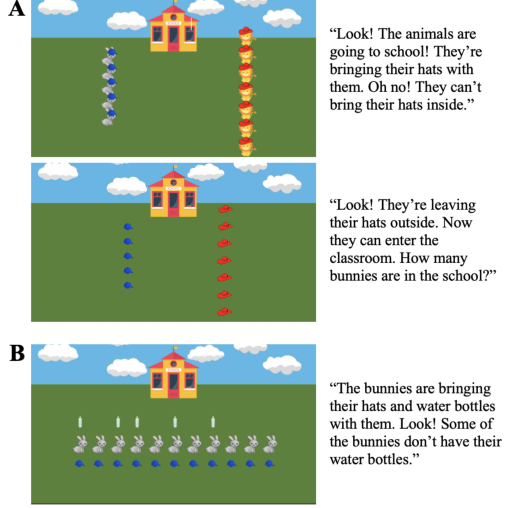
\includegraphics{figs/task_schematic-1} 

}

\caption[A) Materials for Study 1]{A) Materials for Study 1. B) Study 2 includes only 1 animal set with 2 item sets. Left: Visual materials. Right: Corresponding audio description.}\label{fig:task_schematic}
\end{figure}
\end{CodeChunk}

In each critical trial (Figure 1A), participants saw two unequal groups
of animals (e.g., 5 bunnies and 7 lions), each on one side of the
screen. Each animal group was shown in 1-to-1 correspondence with an
item set (e.g., 5 bunnies -- 5 blue hats vs.~7 lions -- 7 pink red
hats). Animal and item sets were organized in a line with equal spacing
to facilitate element tracking and counting. The animals then put down
their items and disappeared into a building. Participants were then
asked for the number of one set of animals (e.g., ``How many bunnies are
in the school?''). We reasoned that if children recognized that sets in
1-to-1 correspondence share the same number, they should use the correct
items to infer the number of animals (e.g., counting the blue hats when
asked about the bunnies). Participants were encouraged to point and
explicitly count the items. If counting resulted in a different
response, we analyzed the final count. Participants were allowed one
opportunity to fix a wrong response.

Participants saw six critical trials in total: three small-set trials
where sets \textless{} 4, and three large-set trials where sets
\textgreater{} 4. Participants saw one out of six pseudo-randomized
trial orders. Trials were counterbalanced for the target animals, side
of set appearance, and which animal set is larger.

\vspace{10pt}

\noindent \textbf{\emph{Highest Count.}} This task was included as a
general proxy of counting experience, to allow us to differentiate
between CP knowers with different degrees of counting expertise.
Participants were asked to ``count as high as {[}they{]} can,''
beginning from one, and prompted once after they stopped to keep
counting. We recorded the highest number they reached without errors. As
a preview, Highest Count was not a significant predictor of performance
in either study, so we omitted results related to this measure for the
purposes of this short paper.

\hypertarget{results-discussion}{%
\subsection{Results \& Discussion}\label{results-discussion}}

Our primary question was whether CP knowers were more likely to succeed
at the Cardinal Extension task compared to subset knowers across both
small and large sets. We first asked whether participants selected the
correct set, either by pointing to the set that was equal to the target
animal set, or by giving the correct count for the target animal
set\footnote{We assumed that children would not be able to report the correct cardinality without identifying the correct set.}.
Two-tailed one-sample t-tests showed that only CP knowers (\(M\) = 0.88,
\(SD\) = 0.32) performed better than chance at identifying the correct
item set to infer the number of hidden animals (\(t(261) = 19.09\),
\(p < .001\)), and they succeeded for both small and large sets (\(p\)s
\textless{} .001). Meanwhile, subset knowers (\(M\) = 0.49, \(SD\) =
0.50) performed at chance (\(t(227) = -0.40\), \(p = .692\)), and failed
to identify the correct set for both small and large sets (\(p\)s
\textgreater{} .05) (Figure 2A). Additionally, there was variability in
CP knowers' performance: out of 44 CP knowers, only 26 (59.09\%)
succeeded in identifying the correct set (either by attempting to count
the correct set, or giving the correct numerical response without
counting) in all six trials (binomial \(p\) \textless{} .05). Three CP
knowers (6.82\%) succeeded in only half of the trials or fewer. These
results provide evidence that the ability to reason about cardinal
extension does not develop when the CP is acquired, but rather after the
CP knowledge stage.

In order to further analyze the effect of CP knowledge on cardinal
extension performance, we constructed generalized mixed-effects logistic
regression models (GLMMs) predicting correct set selection with age
(z-scored), set size (Small/Large), knower level (CP knowers/Subset
knowers), and knower level*set size interaction as fixed effects. We
compared all models against a base model that included only age and set
size as predictors. All models included by-subject and by-item random
intercepts.

\begin{CodeChunk}
\begin{figure}[tb]

{\centering 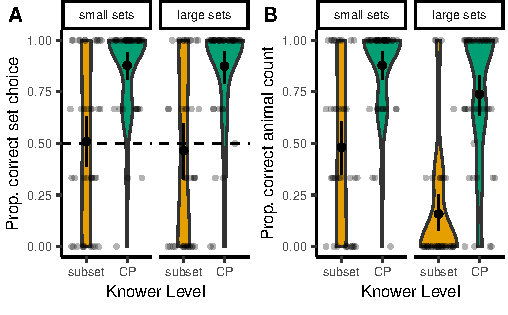
\includegraphics{figs/study1-figure-1} 

}

\caption[Each dot represents a participant]{Each dot represents a participant. The width of the shaded area of violin plots represents the proportion of the data located there. A) Proportion of correct item set choice by participant against knower level. Horizontal dashed line indicates performance at chance = 0.50. B) Proportion of correct numerical response by participant against knower level.}\label{fig:study1-figure}
\end{figure}
\end{CodeChunk}

Our base model showed a significant effect of age (\(\beta\) = 1.67,
95\% CI = {[}1.14, 2.19{]}, \(p < .001\)), with older children
performing better than younger children. Set size (small vs large sets)
did not further explain variation in performance (\(p = .504\)).
Exploratory models analyzing subset knowers and CP knowers separately
showed that this age effect was driven by only subset knowers (\(\beta\)
= 1.56, 95\% CI = {[}0.85, 2.26{]}, \(p < .001\)). Age did not predict
performance in the CP knower group (\(p = .210\)). Adding knower level
as a predictor significantly improved the fit of the model
(\(\chi^2\)(1) = 6.98, \(p = .008\)), and revealed that CP knowers were
significantly more likely than subset knowers to select the correct set,
even when controlling for age (\(\beta\)\(_{CP}\) = 1.43, 95\% CI =
{[}0.37, 2.50{]}, \(p = .008\)). This model also showed a significant
effect of age (\(\beta\) = 1.18, 95\% CI = {[}0.61, 1.75{]},
\(p < .001\)) but not of set size (\(p = .501\)). Adding knower
level*set size interaction did not further improve the model
(\(p = .663\)).

In contrast to these initial analyses in which we considered success in
the task as choosing the correct set corresponding to the hidden
animals, in the next analysis we analyzed performance based on whether
participants both choose the correct set, and correctly inferred the
number of the hidden animal set by counting the correct item set. This
is a more conservative measure of cardinal extension, because success
requires not only attending to the equality of the animal and item sets,
but also counting the selected item set accurately. We constructed
another set of GLMMs with the same fixed and random effect structure as
above to predict children's success in inferring the correct number of
animals.

The model that best explained the data included age, knower level, set
size, and knower level*set size interaction as predictors (compared
against base model with only age and set size: \(\chi^2\)(2) = 20.34,
\(p < .001\); compared against model with age, set size and knower
level: \(\chi^2\)(1) = 4.77, \(p = .029\)). CP knowers were
significantly better at determining the correct number of animals
(\(\beta\)\(_{CP}\) = 1.53, 95\% CI = {[}0.27, 2.78{]}, \(p = .017\)),
as were older children (\(\beta\) = 1.15, 95\% CI = {[}0.55, 1.76{]},
\(p < .001\)). We also found an effect of Set Size with children more
likely to provide the correct numerical response in trials with small
sets compared to those with large sets (\(\beta\)\(_{large}\) = -2.59,
95\% CI = {[}-3.66, -1.52{]}, \(p < .001\)). Additionally, the knower
level*set size interaction effect was significant, where subset knowers
showed a larger difference in performance between small and large trials
compared to CP knowers (\(\beta\)\(_{CP*large}\) = 1.28, 95\% CI =
{[}0.11, 2.45{]}, \(p = .032\)) (Figure 2B).

\hypertarget{study-2-is-cp-knowers-success-in-cardinal-extension-based-on-exact-equality}{%
\section{Study 2: Is CP knowers' success in cardinal extension based on
exact
equality?}\label{study-2-is-cp-knowers-success-in-cardinal-extension-based-on-exact-equality}}

Study 1 showed that CP knowers are able to reason that sets that are
equal in number can be labeled by the same number word. However, it
leaves open how CP knowers might achieve this. One possibility is that
they select the correct item set through noticing a 1-to-1
correspondence between items and animals (e.g., bunnies and hats).
Alternatively, they might compare the approximate quantity of these sets
(e.g., `approximately seven' bunnies and `approximately seven' hats).
They might also succeed by simply noting the association between items
and animals without attending to cardinality at all (e.g., the bunnies
appeared with blue hats, therefore, count the blue hats).

To probe whether CP knowers use exact or approximate quantities in
reasoning about cardinal extension, and to eliminate the possibility of
using identity associations between animals and items, we conducted a
follow-up study that paired one animal set with two item sets in varying
ratios. One item set was in 1-to-1 correspondence with the animal set.
The distractor item set differed in either a perceptually discriminable
manner (e.g., 5 hats - 10 bunnies), or were off by one in quantity and
thus not discriminable (e.g., 9 hats - 10 bunnies). If CP knowers
succeed in cardinal extension through reasoning about 1-to-1
correspondence they should succeed in both cases. However, if they used
approximate quantities, they would succeed in trials with discriminable
ratios, but not in the off-by-one trials.

\hypertarget{methods-1}{%
\subsection{Methods}\label{methods-1}}

\hypertarget{participants-1}{%
\subsubsection{Participants}\label{participants-1}}

A preregistration is available at \url{https://osf.io/zrsw2}. Eighty
children were recruited from preschools and a children's museum in the
US. Given the failure of subset knowers in Study 1, all participants
were CP knowers who spoke English as a primary language. We excluded two
participants who missed more than one trial of the Cardinal Extension
task based on preregistered criteria. We also excluded 18 trials where
participants started counting before the prompt. Our final sample
included 78 CP knowers (43F, 35M; \(M_{age}\) = 4.68 {[}3.29; 5.98{]};
\(SD_{age}\) = 0.71).

\hypertarget{materials-procedure-1}{%
\subsubsection{Materials \& Procedure}\label{materials-procedure-1}}

Participants were given a Give-N task and a Highest Count task following
the procedure from Study 1. To be confident that we included only CP
knowers, we used a more conservative criterion for the Give-N task and
classified children as CP knowers only if they succeeded at constructing
sets of ``six'' two out of three times. Only children who were CP
knowers in the Give-N task proceeded to the Cardinal Extension task.

\textbf{\emph{Cardinal Extension.}} Materials and procedure were similar
to Study 1, with any differences noted. In the familiarization phase,
participants saw an additional trial with three animals (in this study,
only bunnies), but only two of them had items and one of them did not.
The bunny missing an item was pointed out to the participant (``This
bunny doesn't have a carrot.'') Participants were also asked to point
and count the number of bunnies for this trial.

In each critical trial, a set of bunnies appeared at the bottom of the
screen with two sets of items (Figure 1B). One set of items (the target
set) was exactly equal to the number of bunnies, and the other set (the
distractor set) had fewer items. The audio description highlighted the
violation of 1-to-1 correspondence between the distractor set and the
target set in all conditions, and was accompanied by gestures to the
bunnies that were missing items (e.g., `Some of the bunnies don't have
their hats.'). The bunnies then put down each item in each set one at a
time, further emphasizing the 1-to-1 correspondence between the bunnies
and the target set and the mismatch with the distractor set. Like Study
1, the bunnies then disappeared into a building, leaving their items
behind. Participants were then asked for the number of bunnies. If
children use 1-to-1 to reason about exact equality, they should use only
the target set to infer the number of bunnies across conditions. If
participants did not respond, did not overtly count, or made a counting
mistake, they received prompts from the experimenter as described in
Study 1.

Participants saw nine trials in total: three small-set trials where sets
\textless{} 4, and six large-set trials where sets \textgreater{} 4.
Large-set trials included three with discriminable ratios (Large-DR)
where the ratio between the bunnies and the distractor item set was
\textgreater= 2, and three with non-discriminable ratios (Large-NR)
where the distractor set had one fewer item than the number of bunnies.
Participants saw one out of four pseudo-randomized trial orders and item
pairings. The trials were partially-counterbalanced for order and
location of item sets.

\hypertarget{results-discussion-1}{%
\subsection{Results \& Discussion}\label{results-discussion-1}}

Our primary question was whether CP knowers were equally likely to
choose the correct set to infer the number of bunnies across trials of
different set sizes and ratios. Similar to the analysis for the previous
study, we first looked at cardinal extension performance as indexed by
whether the participant selected the correct set, either by pointing to
the correct set or giving the correct number. Two-tailed one-sample
t-tests showed that overall performance was better than chance
(\(t(683) = 10.17\), \(p < .001\)). However, only performance in small
trials (\(M\) = 0.81, \(SD\) = 0.39) and large-DR trials (\(M\) = 0.69,
\(SD\) = 0.46) were better than chance (small trials:
\(t(228) = 12.07\), \(p < .001\), large-DR trials: \(t(225) = 6.34\),
\(p < .001\)). In large-NR trials (\(M\) = 0.54, \(SD\) = 0.50), CP
knowers performed at chance (\(t(228) = 1.12\), \(p = .262\)) (Figure
3). This suggests that CP knowers relied on approximate number
representations to complete the task, but failed whenever 1-to-1
correspondence was required to differentiate sets.

\begin{CodeChunk}
\begin{figure}[h]

{\centering 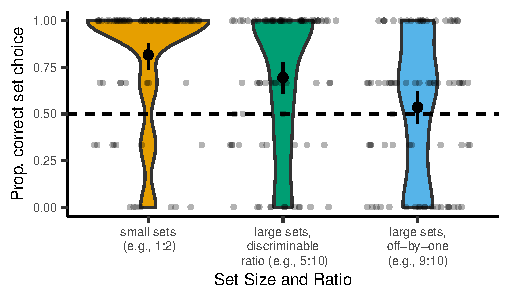
\includegraphics{figs/study2-figure-1} 

}

\caption[Proportion of correct item set choice by participant against trial type]{Proportion of correct item set choice by participant against trial type. Each dot represents a participant. Horizontal dashed line indicates performance at chance = 0.50.}\label{fig:study2-figure}
\end{figure}
\end{CodeChunk}

To further analyze the effect of trial type on whether participants
selected the correct set, we ran GLMMs predicting correct item set
choice with age (z-scored) and trial type (Small/Large-DR/Large-NR) as
fixed effects. We compared this model against a base model that includes
only age as fixed effects. All models included by-subject and by-item
random intercepts.

We found no effect of age in our base model (\(p = .076\)). When trial
type was included as a fixed effect, we found a significant effect of
trial type (\(\chi^2\)(2) = 40.78, \(p < .001\)), and still no effect of
age (\(p = .078\)). The enhanced model explained significantly more
variation in the observed data compared to the base model in a
likelihood ratio test (\(\chi^2\)(2) = 16.97, \(p < .001\)). \emph{Post
hoc} pairwise comparisons between the three trial types (Small,
Large-DR, Large-NR) with Bonferroni corrections showed that CP knowers
were more likely to succeed in Small trials compared to Large-DR trials
(\(z\) = 3.09, \(p = .006\)) and Large-NR trials (\(z\) = 6.34,
\(p < .001\)). Success in Large-DR trials was also significantly higher
than in Large-NR trials (\(z\) = 3.75, \(p < .001\)).

In addition to simply asking whether children chose the correct set as
the basis for inferring the number of hidden bunnies, we also analyzed
performance based on whether participants both inferred the correct set
and counted it correctly. We constructed another set of GLMMs to predict
this behavior, using the same fixed effects structure as above. All
models included by-subject random intercepts, but we omitted
preregistered by-item random intercepts due to overfitting.

The model that best explained the data included both Age and Trial Type
as predictors (compared against base model with only Age: \(\chi^2\)(2)
= 118.96, \(p < .001\)). Older children were significantly better at
providing the correct number of animals (\(\beta\) = 0.54, 95\% CI =
{[}0.03, 1.05{]}, \(p = .036\)). Children's performance was also
influenced by Trial Type (\(\chi^2\)(2) = 82.19, \(p < .001\)), and
\emph{post hoc} pairwise comparisons with Bonferroni correction showed
the same pattern of success across trial types as the above analysis. CP
knowers were more successful in Small trials compared to Large-DR trials
(\(z\) = 7.15, \(p < .001\)) and Large-NR trials (\(z\) = 8.97,
\(p < .001\)), and success in Large-DR trials was also significantly
more likely than in Large-NR trials (\(z\) = 2.84, \(p = .014\)).

\hypertarget{general-discussion-future-directions}{%
\section{General Discussion \& Future
Directions}\label{general-discussion-future-directions}}

We investigated the role that counting knowledge plays in children's
understanding of exact equality, and in particular that sets in 1-to-1
correspondence should be given the same numerical label. We found three
main results. First, compatible with some previous studies, Study 1
found that CP knowers were more likely than subset knowers to infer that
two sets should receive the same number label only if they are
numerically equal. In fact, subset knowers performed at chance on this
task for both small and large sets. This provides evidence against the
hypothesis that exact number meaning develops even before children learn
the CP. Second, Study 1 found that although many CP knowers made this
inference, many also failed, suggesting that this understanding is not
the product of acquiring the CP. Third, Study 2 found that although CP
knowers succeeded at cardinal extension for small sets within the
subitizable range and large sets with perceptually discriminable ratios,
they failed to use 1-to-1 correspondence as a cue to exact equality.
This suggests that CP knowers' initial understanding of cardinal
extension is driven by sensitivity to approximate quantities, not 1-to-1
correspondence.

These results call into question the hypothesis that understanding exact
number meaning occurs when the CP is acquired through a bootstrapping
process where children notice an analogical mapping between counting up
the count list and adding one item to a set (Carey, 2004, 2009).
Therefore, learning the CP supports the inference that only sets in
one-to-one correspondence are equinumerous and can be denoted by the
same number word (Le Corre \& Carey, 2007). Yet our data showed that
children who know the CP performed at chance for perceptually
non-discriminable ratios that are differentiated by violations of 1-to-1
correspondence. This suggests that understanding of how number words
encode exact equality continues to develop well after children master
the counting procedures required to become a CP-knower.

While our results are broadly consistent with some previous findings, we
also introduce several new findings to the literature, which may at
first appear to conflict with some past studies. For example, our
finding that CP knowers extend cardinal labels to two sets even if they
violate one-to-one correspondence seems, at first, to be at odds with
previous studies that document an ability among CP knowers to judge that
sets that differ by just 1 item should be labeled by different number
words (Sarnecka \& Gelman, 2004; Sarnecka \& Wright, 2013). However,
like our study, these previous studies also found variability in CP
knowers' performance, suggesting that many CP knowers fail to recognize
that equinumerous sets should receive the same label. Also, it's unclear
from past studies whether these children who used different labels for
sets with off-by-one difference were sensitive to exact equality, or
were using a pragmatic principle of contrast such as ``different
referents get different labels'' (see Brooks et al., 2013).

One question that arises from our results is why CP knowers succeed at
constructing large sets that are off-by-one (e.g., `five' and `six' fish
in the Give-N task), yet failed to understand that two sets have a
different number of items if they do not exhibit 1-to-1 correspondence.
One possibility, proposed by Davidson et al. (2012), is that CP knowers
have acquired the ability to construct large sets as a rote procedure
and therefore lack adult-like understanding of number words. For
example, when asked to `give six fish,' these CP knowers might follow a
procedure in this form: `Begin counting from one, for each number word
partition one item to a separate set, stop counting at six, and give all
counted objects.' This procedure results in an accurate set of six, but
requires minimal conceptual understanding of the meaning of `six' -- for
example, that `six' denotes the same cardinality across any set
constructed following the procedure, or that `six' denotes `exactly
six.' Lacking this understanding, these CP knowers might not realize
that, if two sets stand in 1-to-1 correspondence, then counting one set
indicates the cardinality of the second one. Another possibility,
proposed by Schneider et al. (2022), is that children might know that
two sets are equal only if they stand in 1-to-1 correspondence but lack
a reliable procedure for verifying this property for large sets.
Schneider et al. (2022) argued that counting provides a procedure that
establishes 1-to-1 correspondence in a memory-free manner: as each item
is counted, it is tagged with a number word and removed from further
consideration (e.g., by setting it aside). Perhaps when children
understand this 1-to-1 verification procedure, they extend the ability
to sequentially map labels-to-objects to the problem of mapping
objects-to-objects in sequence, a skill required for verifying 1-to-1
correspondence in large sets.

Regardless of why some CP knowers fail at cardinal extension, it seems
likely experience with counting plays a role in overcoming these
challenges. Perhaps as children gain more counting experience, they come
to realize that violations of 1-to-1 between count words and items
results in different numerical labels. More exposure to counting might
also lead children to notice that adding or removing an item from a set
results in a different cardinality. Further research is needed to
investigate whether variability in cardinal extension performance among
CP knowers might be explained by differing understanding of the counting
procedures and its conceptual principles.

\hypertarget{acknowledgements}{%
\section{Acknowledgements}\label{acknowledgements}}

This research was funded by a National Science Foundation award
(\#2000827) to DB. We thank the participants, their parents, preschool
teachers and directors, and the Fleet Science Center in San Diego, and
also thank Elizabeth Hernandez and Urvi Maheshwari for assistance with
data collection. We are grateful for the feedback from Rose M. Schneider
and the members of the Language and Development Lab at UC San Diego.

\hypertarget{references}{%
\section{References}\label{references}}

\setlength{\parindent}{-0.1in} 
\setlength{\leftskip}{0.125in}

\noindent

\hypertarget{refs}{}
\begin{CSLReferences}
\leavevmode\vadjust pre{\hypertarget{ref-boolos1986}{}}%
Boolos, G. (1986). Saving {Frege} from contradiction. \emph{Proceedings
of the Aristotelian Society}, \emph{87}, 137--151.

\leavevmode\vadjust pre{\hypertarget{ref-brooks2013}{}}%
Brooks, N., Audet, J., \& Barner, D. (2013). Pragmatic inference, not
semantic competence, guides 3-year-olds' interpretation of unknown
number words. \emph{Developmental Psychology}, \emph{49}(6), 1066.
\url{https://doi.org/10.1037/a0029384}

\leavevmode\vadjust pre{\hypertarget{ref-carey2004}{}}%
Carey, S. (2004). Bootstrapping \& the origin of concepts.
\emph{Daedalus}, \emph{133}, 59--68.
\url{https://doi.org/10.1162/001152604772746701}

\leavevmode\vadjust pre{\hypertarget{ref-carey2009}{}}%
Carey, S. (2009). Where {Our} {Number} {Concepts} {Come} {From}.
\emph{The Journal of Philosophy}, \emph{106}(4), 220--254.
\url{https://doi.org/10.5840/jphil2009106418}

\leavevmode\vadjust pre{\hypertarget{ref-condry2008}{}}%
Condry, K. F., \& Spelke, E. S. (2008). The development of language and
abstract concepts: {The} case of natural number. \emph{Journal of
Experimental Psychology: General}, \emph{137}(1), 22--38.
\url{https://doi.org/10.1037/0096-3445.137.1.22}

\leavevmode\vadjust pre{\hypertarget{ref-cordes2001}{}}%
Cordes, S., Gelman, R., Gallistel, C. R., \& Whalen, J. (2001).
Variability signatures distinguish verbal from nonverbal counting for
both large and small numbers. \emph{Psychonomic Bulletin \& Review},
\emph{8}, 698--707. \url{https://doi.org/10.3758/BF03196206}

\leavevmode\vadjust pre{\hypertarget{ref-davidson2012}{}}%
Davidson, K., Eng, K., \& Barner, D. (2012). Does learning to count
involve a semantic induction? \emph{Cognition}, \emph{123}(1), 162--173.
\url{https://doi.org/10.1016/j.cognition.2011.12.013}

\leavevmode\vadjust pre{\hypertarget{ref-decock2008}{}}%
Decock, L. (2008). Neo-fregeanism naturalized: The role of one-to-one
correspondence in numerical cognition. \emph{Behavioral and Brain
Sciences}, \emph{31}(6), 648--649.
\url{https://doi.org/10.1017/S0140525X08005645}

\leavevmode\vadjust pre{\hypertarget{ref-feigenson2004}{}}%
Feigenson, L., Dehaene, S., \& Spelke, E. (2004). Core systems of
number. \emph{Trends in Cognitive Sciences}, \emph{8}(7), 307--314.
\url{https://doi.org/10.1016/j.tics.2004.05.002}

\leavevmode\vadjust pre{\hypertarget{ref-frege1880}{}}%
Frege, G. (1880). \emph{Booles rechnende logik und die begriffsschrift}.

\leavevmode\vadjust pre{\hypertarget{ref-frege1884}{}}%
Frege, G. (1884). \emph{Die grundlagen der arithmetik: Eine logisch
mathematische untersuchung über den begriff der zahl}. W. Koebner.

\leavevmode\vadjust pre{\hypertarget{ref-frydman1988}{}}%
Frydman, O., \& Bryant, P. (1988). Sharing and the understanding of
number equivalence by young children. \emph{Cognitive Development},
\emph{3}(4), 323--339.
\url{https://doi.org/10.1016/0885-2014(88)90019-6}

\leavevmode\vadjust pre{\hypertarget{ref-izard2014}{}}%
Izard, V., Streri, A., \& Spelke, E. S. (2014). Toward exact number:
{Young} children use one-to-one correspondence to measure set identity
but not numerical equality. \emph{Cognitive Psychology}, \emph{72},
27--53. \url{https://doi.org/10.1016/j.cogpsych.2014.01.004}

\leavevmode\vadjust pre{\hypertarget{ref-lecorre2007}{}}%
Le Corre, M., \& Carey, S. (2007). One, two, three, four, nothing more:
An investigation of the conceptual sources of the verbal counting
principles. \emph{Cognition}, \emph{105}(2), 395--438.
\url{https://doi.org/10.1016/j.cognition.2006.10.005}

\leavevmode\vadjust pre{\hypertarget{ref-le2024}{}}%
Le, K. N., Schneider, R. M., \& Barner, D. (2024). \emph{The development
of cardinal extension: From counting to exact equality}. PsyArXiv.
\url{https://doi.org/10.31234/osf.io/2agtm}

\leavevmode\vadjust pre{\hypertarget{ref-muldoon2003}{}}%
Muldoon, K., Lewis, C., \& Freeman, N. H. (2003). Putting counting to
work: Preschoolers' understanding of cardinal extension.
\emph{International Journal of Educational Research}, \emph{39}(7),
695--718. \url{https://doi.org/10.1016/j.ijer.2004.10.006}

\leavevmode\vadjust pre{\hypertarget{ref-muldoon2005}{}}%
Muldoon, K., Lewis, C., \& Towse, J. (2005). Because it's there! Why
some children count, rather than infer numerical relationships.
\emph{Cognitive Development}, \emph{20}(3), 472--491.
\url{https://doi.org/10.1016/j.cogdev.2005.05.008}

\leavevmode\vadjust pre{\hypertarget{ref-piaget1965}{}}%
Piaget, J. (1965). The stages of the intellectual development of the
child. \emph{Educational Psychology in Context: Readings for Future
Teachers}, \emph{63}(4), 98--106.

\leavevmode\vadjust pre{\hypertarget{ref-russac1978}{}}%
Russac, R. (1978). The relation between two strategies of cardinal
number: Correspondence and counting. \emph{Child Development}, 728--735.
\url{https://doi.org/10.2307/1128241}

\leavevmode\vadjust pre{\hypertarget{ref-sarnecka2004}{}}%
Sarnecka, B., \& Gelman, S. A. (2004). Six does not just mean a lot:
Preschoolers see number words as specific. \emph{Cognition},
\emph{92}(3), 329--352.
\url{https://doi.org/10.1016/j.cognition.2003.10.001}

\leavevmode\vadjust pre{\hypertarget{ref-sarnecka2013}{}}%
Sarnecka, B., \& Wright, C. E. (2013). The {Idea} of an {Exact}
{Number}: {Children}'s {Understanding} of {Cardinality} and
{Equinumerosity}. \emph{Cognitive Science}, \emph{37}(8), 1493--1506.
\url{https://doi.org/10.1111/cogs.12043}

\leavevmode\vadjust pre{\hypertarget{ref-schneider2022}{}}%
Schneider, R. M., Brockbank, E., Feiman, R., \& Barner, D. (2022).
Counting and the ontogenetic origins of exact equality.
\emph{Cognition}, \emph{218}, 104952.
\url{https://doi.org/10.1016/j.cognition.2021.104952}

\leavevmode\vadjust pre{\hypertarget{ref-slusser2011}{}}%
Slusser, E. B., \& Sarnecka, B. W. (2011). Find the picture of eight
turtles: A link between children's counting and their knowledge of
number word semantics. \emph{Journal of Experimental Child Psychology},
\emph{110}(1), 38--51. \url{https://doi.org/10.1016/j.jecp.2011.03.006}

\leavevmode\vadjust pre{\hypertarget{ref-sophian1995}{}}%
Sophian, C., Wood, A. M., \& Vong, K. I. (1995). Making numbers count:
The early development of numerical inferences. \emph{Developmental
Psychology}, \emph{31}(2), 263.
\url{https://doi.org/10.1037/0012-1649.31.2.263}

\leavevmode\vadjust pre{\hypertarget{ref-whalen1999}{}}%
Whalen, J., Gallistel, C. R., \& Gelman, R. (1999). Nonverbal counting
in humans: The psychophysics of number representation.
\emph{Psychological Science}, \emph{10}(2), 130--137.
\url{https://doi.org/10.1111/1467-9280.00120}

\leavevmode\vadjust pre{\hypertarget{ref-wynn1990}{}}%
Wynn, K. (1990). Children's understanding of counting. \emph{Cognition},
\emph{36}(2), 155--193.
\url{https://doi.org/10.1016/0010-0277(90)90003-3}

\leavevmode\vadjust pre{\hypertarget{ref-wynn1992}{}}%
Wynn, K. (1992). Children's acquisition of the number words and the
counting system. \emph{Cognitive Psychology}, \emph{24}(2), 220--251.
\url{https://doi.org/10.1016/0010-0285(92)90008-P}

\end{CSLReferences}

\bibliographystyle{apacite}


\end{document}
